% Chapter 5

\chapter{Examples}

\label{ch:examples}

The following pages demonstrate a few code examples of how to use the
\tangible{} library.

%----------------------------------------------------------------------------------------

\section{A Simple Tower}\label{sec:tower}

This example describes a simple round tower where the radius of the layers
corresponds to the datapoint. The dataset describes the number of web site
visits on \url{http://blog.dbrgn.ch/} during the month of September 2013. The
value range is normalized to a range between 10 and 50 using a linear scale.

\vspace{.5\baselineskip}
\begin{pythoncode}
from tangible import scales
from tangible.shapes.vertical import CircleTower1D
from tangible.backends.openscad import OpenScadBackend

# Normalize raw data
visits = [53, 69, 86, 92, 81, 76, 37, 36, 62, 76, 72, 67, 55, 61, 54,
          72, 92, 84, 78, 75, 45, 48, 85, 81, 83, 69, 68, 66, 62, 115]
scale = scales.linear([min(visits), max(visits)], [10, 50])
datapoints = map(scale, visits)

# Create shape
tower = CircleTower1D(datapoints, layer_height=10)

# Render OpenSCAD code
code = tower.render(backend=OpenScadBackend)
print code
\end{pythoncode}
\vspace{.5\baselineskip}

\begin{figure}[H]
	\centering
	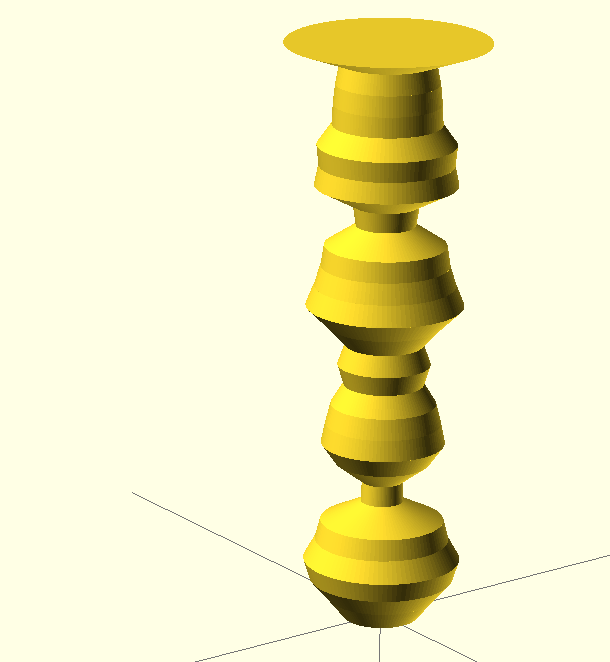
\includegraphics[height=.25\textheight]{images/tower.png}
	\caption{A CircleTower1D shape}
	\label{img:tower}
\end{figure}

%----------------------------------------------------------------------------------------

\newpage
\section{Multi Dimensional Data}\label{sec:multidimensional}

Here we have two dimensional data, represented as two lists of integers. The
first list should be mapped to the angle of the ``pie slices'', while the second
list should be mapped to the height of each slice. Additionally, we'll add a
center radius to make the model look like a donut, and we'll explode the slices.

\vspace{.5\baselineskip}
\begin{pythoncode}
from tangible.shapes.pie import AngleHeightPie2D
from tangible.backends.openscad import OpenScadBackend

# Data
datapoints = [
    [30, 30, 5, 5, 20], # Angle
    [18, 23, 20, 15, 10], # Height
]

# Create shape
pie = AngleHeightPie2D(datapoints, inner_radius=4, explode=1)

# Render OpenSCAD code
code = pie.render(backend=OpenScadBackend)
print code
\end{pythoncode}
\vspace{.5\baselineskip}

\begin{figure}[H]
	\centering
	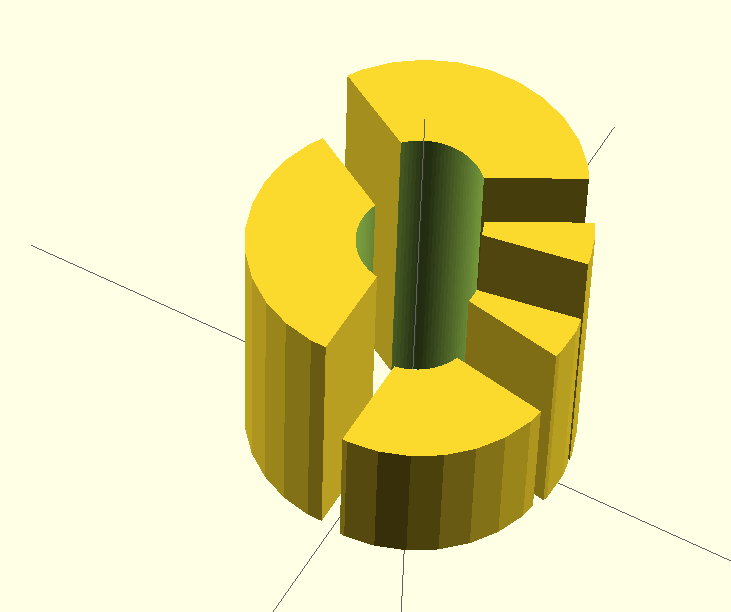
\includegraphics[height=.3\textheight]{images/angle_pie.png}
	\caption{An AnglePie2D shape}
	\label{img:angle_pie}
\end{figure}

%----------------------------------------------------------------------------------------

\newpage
\section{Reading Data from CSV}\label{sec:csv}

Often the data that you want to visualize is not already available as a Python
datastructure, but in formats like JSON or CSV. Here's a small example where
website visitor data is read from the CSV exported by Google Analytics. Then the
number of visits and the average visit duration are mapped to the distance
between opposing corners of a rhombus tower.

\vspace{.5\baselineskip}
\begin{pythoncode}
import csv
from datetime import timedelta
from tangible.shapes.vertical import RhombusTower2D
from tangible.backends.openscad import OpenScadBackend

# Read data into list
datapoints = [[], []]
with open('analytics-sep-13.csv', 'r') as datafile:
    reader = csv.DictReader(datafile)
    for row in reader:
        datapoints[0].append(int(row['Visits']))
        h, m, s = map(int, row['AvgDuration'].split(':'))
        duration = timedelta(hours=h, minutes=m, seconds=s)
        datapoints[1].append(duration.total_seconds())

# Create shape
tower = RhombusTower2D(datapoints, layer_height=10)

# Render OpenSCAD code
code = tower.render(backend=OpenScadBackend); print code
\end{pythoncode}
\vspace{.5\baselineskip}

\noindent Here are the CSV contents:

\vspace{.5\baselineskip}
\begin{minted}[frame=lines,framesep=2mm,samepage=true,fontsize=\footnotesize]{text}
Day,Visits,AvgDuration
9/1/13,53,00:00:51
9/2/13,69,00:01:01
9/3/13,86,00:01:24
...
\end{minted}
\vspace{.5\baselineskip}

\noindent And the resulting shape:

\begin{figure}[H]
	\centering
	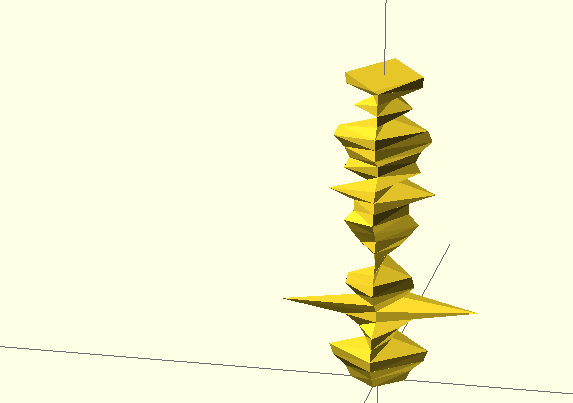
\includegraphics[height=.20\textheight]{images/csv.png}
	\caption{A RhombusTower2D shape from CSV data}
	\label{img:angle_pie}
\end{figure}


%----------------------------------------------------------------------------------------

\newpage
\section{Grouped Data}\label{sec:tower}

Some one dimensional datasets does not work well when visualized directly. An
example would be website visitor statistics during a full year, a single bar
graph would be much too wide. But by grouping the data from example
\ref{sec:csv} into months, a \texttt{BarsND} graph can be constructed:

\vspace{.5\baselineskip}
\begin{pythoncode}
import csv
from itertools import chain
from tangible import scales
from tangible.shapes.bars import BarsND
from tangible.backends.openscad import OpenScadBackend

# Read data into list
datapoints = [list() for i in xrange(9)]
with open('analytics-full-13.csv', 'r') as datafile:
    reader = csv.DictReader(datafile)
    for row in reader:
        date = row['Day']
        month = int(date.split('/', 1)[0])
        visits = int(row['Visits'])
        datapoints[month - 1].append(visits)

# Normalize data
all_datapoints = list(chain.from_iterable(datapoints))
scale = scales.linear([min(all_datapoints), max(all_datapoints)],
                      [10, 150])
datapoints = map(lambda x: map(scale, x), datapoints)

# Create shape
bars = BarsND(datapoints, bar_width=7, bar_depth=7)

# Render OpenSCAD code
code = bars.render(backend=OpenScadBackend); print code
\end{pythoncode}
\vspace{.5\baselineskip}

\begin{figure}[H]
	\centering
	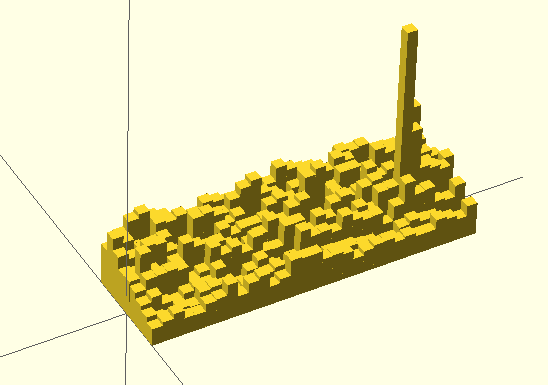
\includegraphics[height=.28\textheight]{images/bars_nd.png}
	\caption{A BarsND shape from CSV data grouped by month}
	\label{img:bars_nd}
\end{figure}

%----------------------------------------------------------------------------------------

\newpage
\section{Creating Custom Shapes from AST}\label{sec:custom_ast}

It's not necessary to rely on the provided shape classes only, you can also
create your own shapes by using the \hyperref[sec:ast]{AST} objects directly.

The easiest and cleanest way to do this, is to create a subclass of the
\texttt{BaseShape} class and to override its \texttt{\_build\_ast} method:

\vspace{.5\baselineskip}
\begin{pythoncode}
from tangible.shapes.base import BaseShape
from tangible import ast
from tangible.backends.openscad import OpenScadBackend

# Create custom shape
class Cogwheel(BaseShape):
    def _build_ast(self):
        cogs = []
        for i in xrange(18):
            cog = ast.Rectangle(2, 2)
            translated = ast.Translate(9.5, -1, 0, cog)
            rotated = ast.Rotate(i * 30, (0, 0, 1), translated)
            cogs.append(rotated)
        return ast.Union([ast.Circle(radius=10)] + cogs)

# Render shape
f = Cogwheel()
code = f.render(backend=OpenScadBackend)
print code
\end{pythoncode}
\vspace{.5\baselineskip}

\begin{figure}[H]
	\centering
	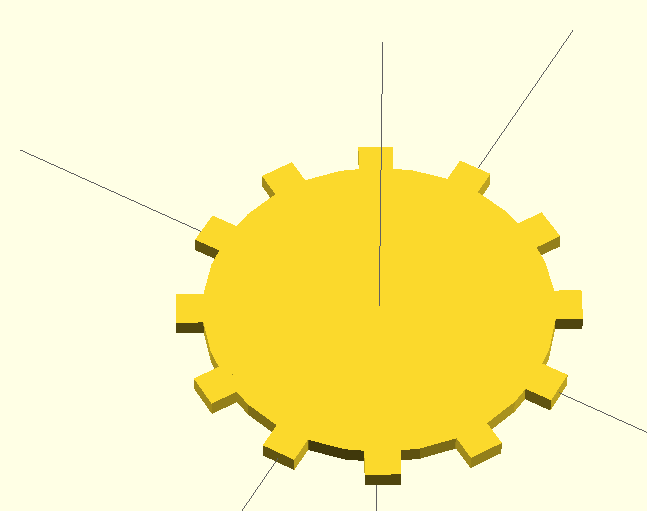
\includegraphics[height=.3\textheight]{images/cogwheel.png}
	\caption{A custom cogwheel shape}
	\label{img:cogwheel}
\end{figure}
